\documentclass{article}
\usepackage{graphicx} % Required for inserting images
\usepackage{amsmath}
\usepackage{amssymb} % used for math symbols
\usepackage{mathtools}
\usepackage{enumitem}
\usepackage{wasysym}
\usepackage{float}
\usepackage{minted}
\usepackage{tikz}
\usepackage{svg}


\title{Computer Grafik Blatt 10}
\date{June 2023}

\begin{document}

\maketitle

\section*{Aufgabe 1.}

\subsection*{(a)}
% include aufgabe1a.pdf
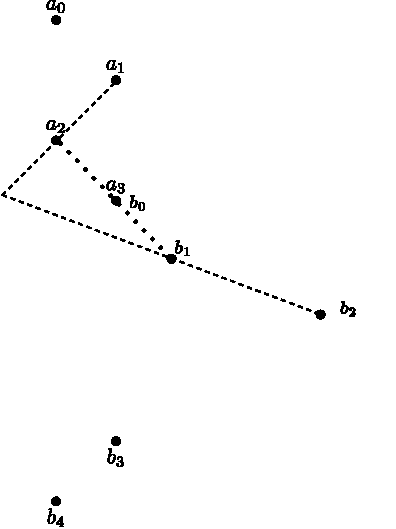
\includegraphics[width=\textwidth]{aufgabe1a.pdf}



\subsection*{(b)}
% lineare Bezierkurve => 2 Punkte
% quadratische Bezierkurve => 3 Punkte
% kubische Bezierkurve => 4 Punkte

% $C^0$-stetig: Der Endpunkt der vorherigen Kurve ist der Anfangspunkt der nächsten Kurve.

$b_0 = a_1 = (4,4)$ \\
$b_1 = (5,5)$, beliebig wählbar \\
$c_1 = (5,5)$ \\
$c_2 = (6,6)$, beliebig wählbar \\

\subsection*{(c)}
$b_0 = a_1 = (4,4)$ \\
\[
    \begin{aligned}
        b_0 &= \frac{1}{2} \cdot (a_0 + b_1) \\
        b_1 &= 2 \cdot b_0 - a_0 \\
        b_1 &= 2 \cdot (4,4) - (3,7) \\
        b_1 &= (8,8) - (3,7) \\
        b_1 &= (5,1)
    \end{aligned}
\]

$c_0 = b_1 = (5,1)$ \\
\[
    \begin{aligned}
        c_1 &= \frac{1}{2} \cdot (b_0 + c_1) \\
        c_1 &= 2 \cdot c_0 - b_0 \\
        c_1 &= 2 \cdot (5,1) - (4,4) \\
        c_1 &= (10,2) - (4,4) \\
        c_1 &= (6,-2)
    \end{aligned}
\]

\subsection*{(d)}
Nicht lösbar.

\subsection*{(e)}

\end{document}
